\section{Durchführung}
\label{sec:durch}
Zur Aufnahme der Temperatur-Strom Kurven wird der in Abbildung \ref{fig:aufbau} skizzierte Aufbau verwendet.

\begin{figure}
    \centering
    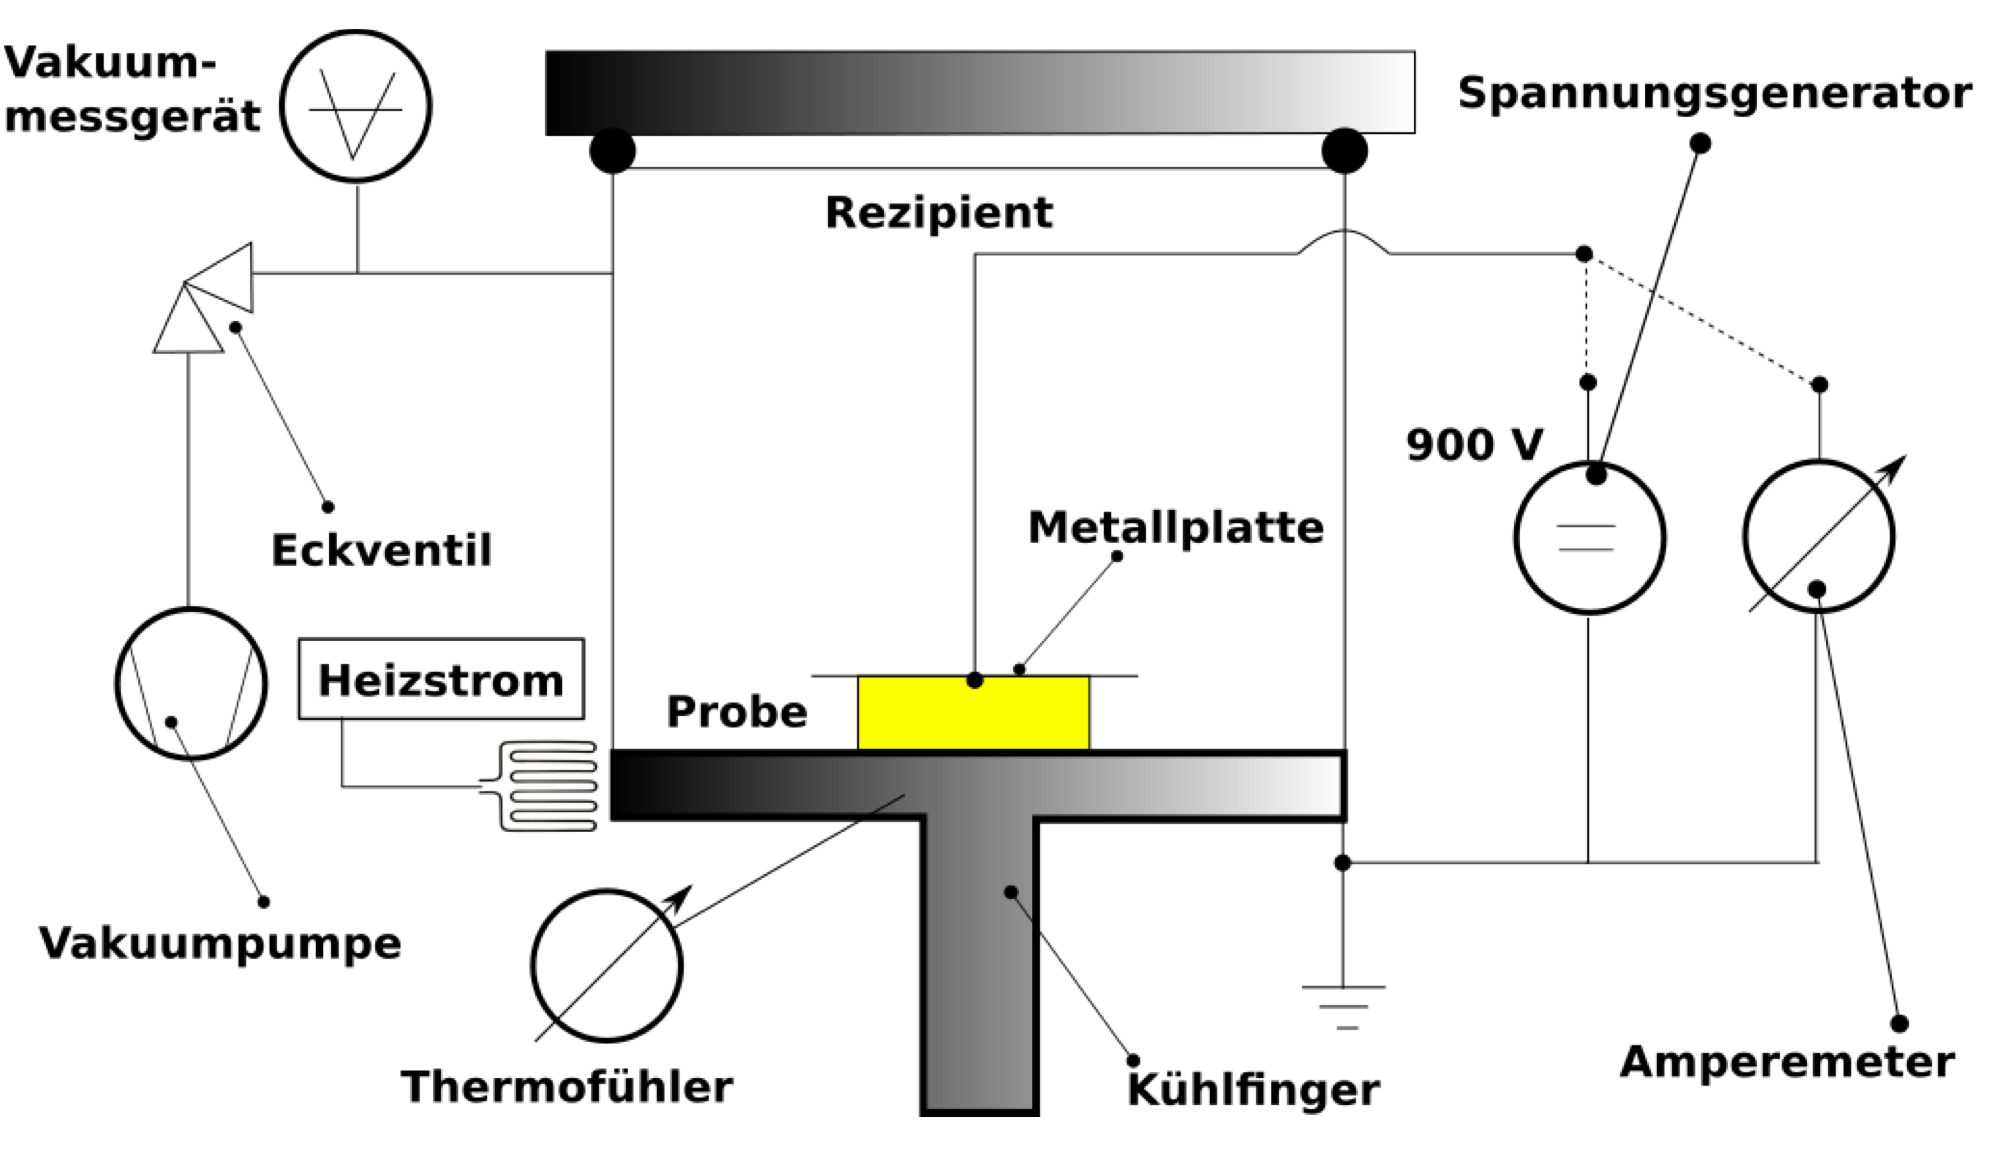
\includegraphics[width=0.75\textwidth]{aufbau.png}
    \caption{Skizzenhafte Darstellung des evakuierten Rezipienten mit einer sich in einem Kondensator befindlichen Probe in Inneren \cite{V48}.}
    \label{fig:aufbau}
  \end{figure}

\noindent
Der Aufbau besteht aus einem evakuiertem Rezipienten, in dem sich die Probe, mit Strontium dotiertes Kaliumbromid, in einem Plattenkondensator befindet.
Der Druck im Rezipienten beträgt 0,01 mbar, was einen Untergrundstrom unterdrückt, der sonst durch das sich in der Luft befindliche Wasser ausgelöst wird.
Die Probe kann durch einen Heizstrom erwärmt werden, wobei die Temperatur mithilfe eines Thermofühlers abgelesen werden kann.
Durch Untersellen eines mit flüssigem Stickstoff gefüllten Dewar-Gefäßes kann die Probe über den Kühlfinger abgekühlt werden. 


\noindent
Um den Depolarisationsstrom zu messen, wird zunächst die Heizspannung auf 60V gestellt und gewartet, bis der Kristall eine Temperatur von 50°C erreicht.
Parallel dazu kann eine Spannung am Plattenkondensator angelegt werden, damit ein elektrisches Feld entsteht nach welchem sich die Dipolmomente ausrichten können.
Wenn der Kristall eine Temperatur von 50°C erreicht hat, wird die Heizspannung ausgeschaltet und das Dewar-Gefäß mit flüssigem Stickstoff unter den Kühlfinger gestellt.
Erreicht der Kristall durch das Abkühlen eine Temperatur von -50°C, wird die Kondensatorspannung abgeschaltet und der Kondensator wird 15 minuten geerdet.
Danach wird der Kondensator an ein Amperemeter angeschlossen und die Heizspannung wird so angelegt, dass eine Heizrate von b=2$\frac{\text{K}}{\text{min}}$ eingehalten wird.
Pro Minute wird die Temperatur des Kristalls und die vom Amperemeter abgelesene Stromstärke aufgenommen, wobei die Heizspannung nachreguliert wird um eine konstante Heizrate einzuhalten.
Die Messung wird beendet, wenn der Kristall eine Temperatur von 50°C erreicht hat.
Es wird erneut eine Kondensatorspannung angelegt und die Messung wird für eine Heizrate von b=1,5$\frac{\text{K}}{\text{min}}$ wiederholt.


